\chapter{Obiettivi della tesi} %\label{1cap:spinta_laterale}
% [titolo ridotto se non ci dovesse stare] {titolo completo}
%

\begin{citazione}
Questo capitolo descrive il cuore dello studio: la definizione degli obiettivi permetterà di delineare le funzionalità chiave che il sistema dovrà implementare per rispondere in modo efficace alle esigenze degli utenti finali.
\end{citazione}
\newpage
\section{Obiettivo della tesi}
Come è stato accennato nei capitoli precedenti, l'obiettivo principale sul quale è stato fondato tutto lo studio presente all'interno di questa tesi, riguarda principalmente l'analisi e lo studio delle prestazioni relative alla sicurezza di particolari flussi di dati i quali posseggono determinati requisiti \emph{time sensitive} che devono essere rispettati affinché possano fornire la piena funzionalità dei sistemi correlati e soprattutto garantire una determinata qualità dei servizi offerti. I flussi definiti saranno posti in analisi tenendo in considerazione del fatto che su di essi impatterà l'utilizzo di diversi protocolli VPN tra cui \emph{WireGuard}. Con questo studio si intende contribuire attivamente alla ricerca, in modo da stabilire chiaramente il comportamento di determinati flussi di dati in relazione anche al protocollo VPN scelto per garantire il giusto grado di sicurezza. 

\section{Identificazione delle funzionalità del dispositivo}
Passiamo ora alla definizione delle diverse funzionalità che il dispositivo in questione dovrà supportare per soddisfare le esigenze degli utenti. Di seguito sono elencate le principali utilità del dispositivo:
\begin{itemize}
    \item Il dispositivo deve fornire la possibilità di eseguire scansioni sui dispositivi connessi alla stessa rete LAN della testbed;
    \item La testbed deve fornire la possibilità connettersi ad un server VPN in modo da poter navigare in modo sicuro ed accedere alle risorse della rete da remoto.
\end{itemize}

\section{Identificazione requisiti non funzionali e di sicurezza}
Ora passiamo alla definizione dei vincoli che descrivono le proprietà e le restrizioni riguardanti il sistema stesso oltreché alle procedure necessarie per evitare la sua compromissione:
\begin{itemize}
    \item Il dispositivo deve essere costantemente alimentato;
    \item Il dispositivo deve autenticare gli utenti prima di permettere l'utilizzo del servizio VPN;
    \item I dati trasmessi tramite canale VPN devono essere crittografati;
    \item Il dispositivo dovrebbe essere fisicamente resistente ad attacchi.
\end{itemize}

\section{Interazione con la API}
In questa sezione sono rappresentate le interazioni tra il sistema ed i principali attori coinvolti nel normale utilizzo. Analizziamo i casi d'uso relativi alle funzionalità da realizzare.

\subsection{Use case modulo scansione}
Il caso d’uso in questione riguarda l’utilizzo del modulo adibito alle scansioni degli \emph{host} presenti nella LAN a cui è connesso il dispositivo da parte del network admin o di chi ne fa le veci.
\begin{figure}[h] 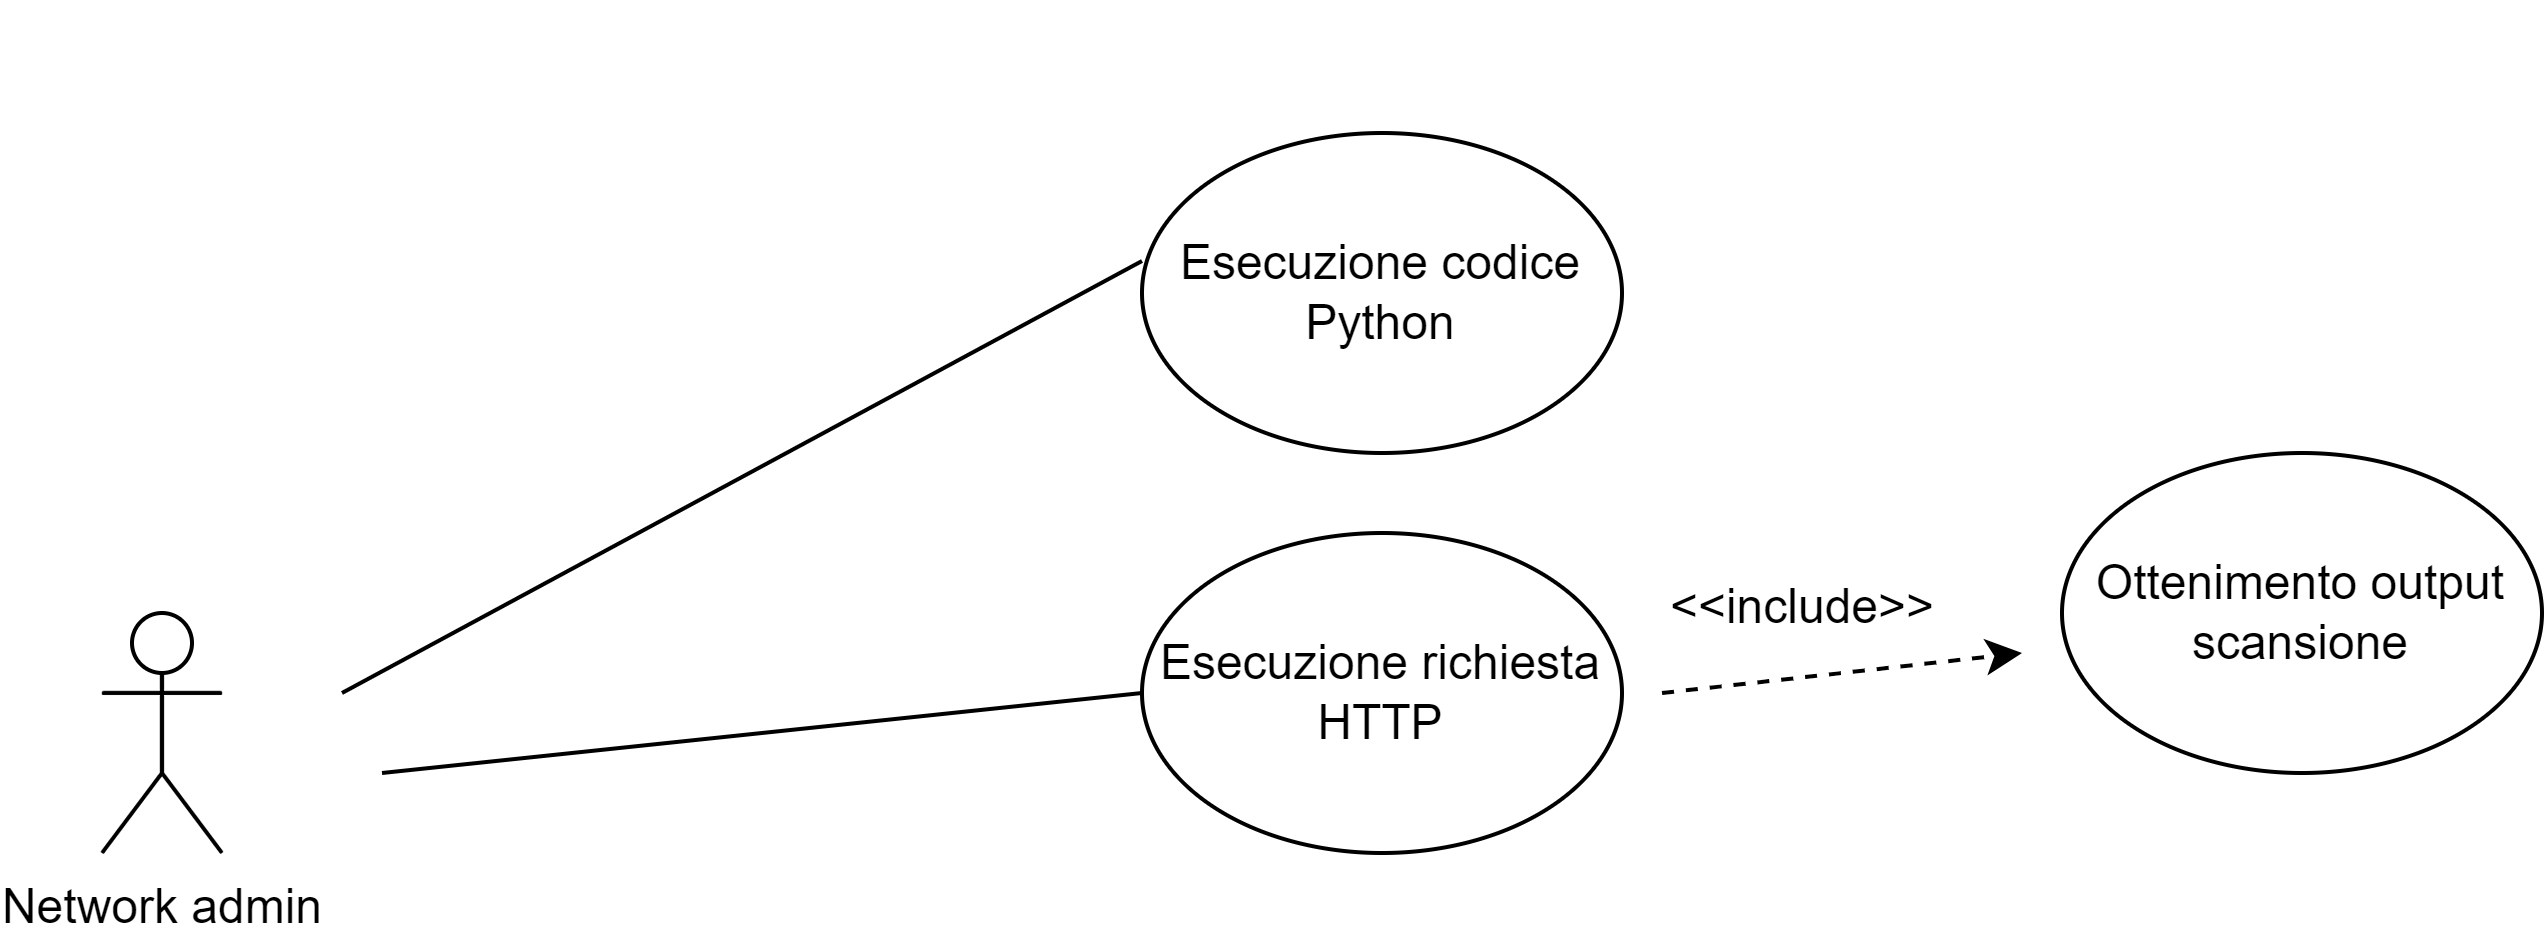
\includegraphics[width=0.7\textwidth] {Tesi magistrale/capitoli/images/use case 1.png}
\centering
\caption{Use case modulo scansione.}
\end{figure}

\subsection{Use case modulo VPN}
Come si evince dall’immagine sottostante, il modulo VPN viene anch’esso gestito da una figura preposta a tale lavoro; mentre i vari client che desiderano connettersi al \emph{server VPN} hanno la possibilità di usufruire del servizio finale cioè entrare a far parte della rete LAN del dispositivo o navigare in modo sicuro.

\begin{figure}[h] 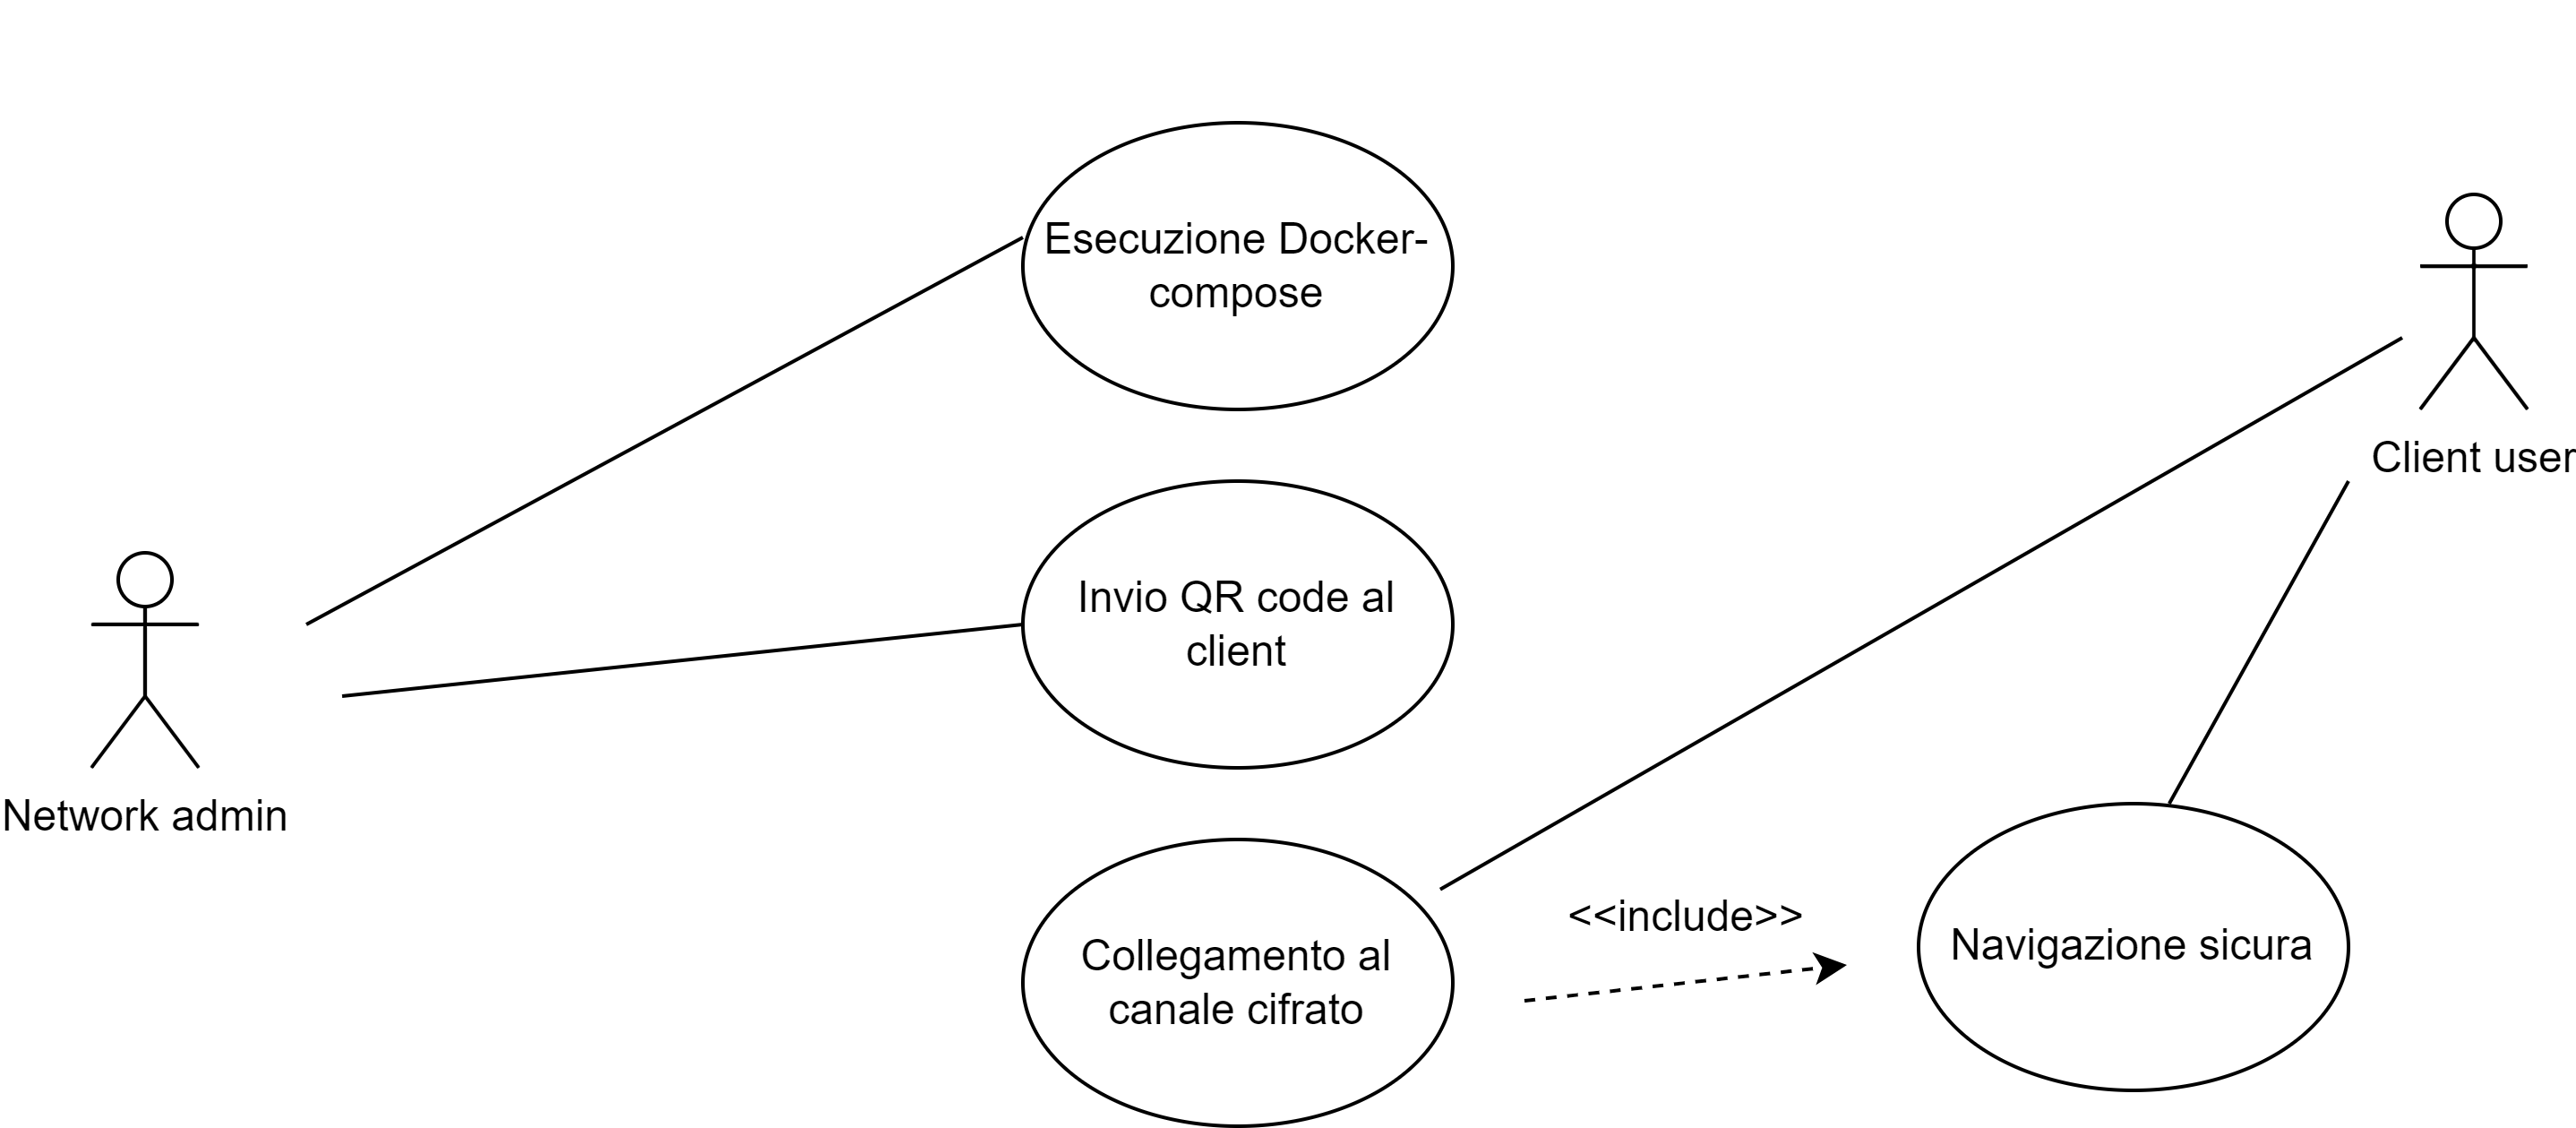
\includegraphics[width=0.7\textwidth] {Tesi magistrale/capitoli/images/use case 2.png}
\centering
\caption{Use case modulo VPN.}
\end{figure}

\section{Conclusioni}
I requisiti raccolti in questa fase saranno successivamente impiegati per la progettazione e l'implementazione del sistema proposto.
